\subsubsection{模型建立}

针对问题一，从产销分段收益和跨期土地约束两个角度建立确定性多期MILP。

\textbf{步骤1 产量与销量线性化}

设$x_{tisj}$为年$t$季次$s$地块$i$种植作物$j$的面积，$z_{tisj}$为对应二元变量。该批次产量为
\begin{equation}
Y_{tisj}=y^0_{g_i s j}x_{tisj}.
\end{equation}
设$q_{tisj}$为按正常价格销售的产量，则
\begin{equation}
0\le q_{tisj}\le Y_{tisj},\qquad
\sum_{i,s}q_{tisj}\le D_j^0.
\end{equation}
当$\alpha=0$时超额产量滞销，当$\alpha=0.5$时超额部分按半价销售。七年目标函数为
\begin{equation}
\max \Pi^{(\alpha)}=
\sum_{t,i,s,j}\Bigl\{p^0_{g_i s j}\Bigl[\alpha y^0_{g_i s j}x_{tisj}+(1-\alpha)q_{tisj}\Bigr]-c^0_{g_i s j}x_{tisj}\Bigr\}.
\end{equation}

\textbf{步骤2 适种与轮作约束}

先按适种规则限定变量域。设地块 $i$ 的类型为 $g_i$，类型 $g$、季次 $s$ 下适种作物集合为 $\mathcal{J}(g,s)$。露地（平旱地、梯田、山坡地）单季适种作物 $1$--$15$ 号；水浇地第一季适种水稻 $16$ 号或蔬菜 $17$--$34$ 号，第二季适种蔬菜 $35$--$37$ 号；普通大棚第一季适种蔬菜 $17$--$34$ 号，第二季适种食用菌 $38$--$41$ 号；智慧大棚两季均适种蔬菜 $17$--$34$ 号。据此仅对 $j\in\mathcal{J}(g_i,s)$ 建立变量 $x_{tisj}$、$z_{tisj}$。

每个地块季次须种满面积（水浇地第二季按模式处理，见下文），并通过下式约束种植活动。
\begin{align}
\sum_{j\in\mathcal{J}(g_i,s)}x_{tisj}&=A_i,\\
\rho A_i z_{tisj}&\le x_{tisj}\le A_i z_{tisj},\\
\sum_{j\in\mathcal{J}(g_i,s)}z_{tisj}&\le3.
\end{align}
其中 $\rho\in\{0,0.1\}$ 为最小面积占比，$3$ 为每地块季次作物数上限，用于量化管理便利。

相邻可种植季内同一作物不能重茬\upcite{capitanescu2017}。对同地块 $i$ 相邻两个季次 $(t,s)$ 与紧随其后的季次 $(t',s')=\mathcal{N}(t,s)$（含跨年边界），若作物 $j$ 在两个季次均适种，则
\begin{equation}
z_{tisj}+z_{t'is'j}\le1,\qquad j\in\mathcal{J}(g_i,s)\cap\mathcal{J}(g_i,s').
\end{equation}
此外，2023 年末季已种的作物在 2024 年首个季次被强制取 $0$，实现与历史种植的衔接。

设 $\mathcal B=\{1,\dots,5\}\cup\{17,\dots,19\}$ 为豆类集合。任意连续三年窗口内每地块豆类累计面积不少于该地块面积，以 2023 年为起点的首个窗口计入 2023 年豆类面积。该约束写为
\begin{equation}
\sum_{\tau=t}^{t+2}\sum_s\sum_{j\in\mathcal B}x_{\tau isj}\ge A_i.
\end{equation}

水浇地以二元变量 $w_{ti}$ 区分模式。其中 $w_{ti}=1$ 为单季水稻，$w_{ti}=0$ 为两季蔬菜。记第一季、第二季分别为季次 $s_1$、$s_2$，则
\begin{align}
z_{tis_1,16}&\le w_{ti},\\
\sum_{j=17}^{34}z_{tis_1 j}&\le3(1-w_{ti}),\\
\sum_{j=35}^{37}z_{tis_2 j}&=1-w_{ti},\\
\sum_{j=35}^{37}x_{tis_2 j}&=A_i(1-w_{ti}).
\end{align}
上式保证水稻模式（$w_{ti}=1$）下第一季只种水稻、第二季空置；蔬菜模式（$w_{ti}=0$）下第一季种蔬菜、第二季在 $35$--$37$ 号中恰选一种并种满。

\textbf{步骤3 求解设置}

模型使用 HiGHS 求解\upcite{huangfu2018}，以 Gap 达到验收线（滞销 3\%、半价 1\%）作为求解质量判据。每个正式方案含 7434 个面积变量、22358 个决策变量和约 $2.0\times10^4$ 至 $2.8\times10^4$ 条约束，单次求解耗时约 3 至 179 秒，均在 300 秒时限内完成。

\subsubsection{模型求解}

正式滞销表采用$\rho=0$配置，累计净收益为4041.72万元，MIP Gap为2.126\%；正式半价销售表采用$\rho=0.1$配置，累计净收益为6351.02万元，MIP Gap为0.739\%。两份正式方案的硬约束违反数均为0。

对比规则轮作基线，主方法的收益更高。滞销模式下基线累计净收益为2195.33万元，主方法高出约84\%；半价模式下基线为3900.24万元，主方法高出约63\%。这一优势来自全局优化对地块间种植结构的统筹调度，而非单季利润的简单追逐。种植结构上，滞销模式保留全部41种作物（前三作物面积占比约42\%），半价模式收敛至24种作物（前三作物面积占比约44\%），均未出现单一作物占据绝大面积或结构退化的现象。销售规则解释了两种结构的差异。半价销售使超额产量仍产生一半收益，模型因此倾向集中种植高利润的蔬菜与食用菌；滞销模式下超额产量无收益，保留作物多样性可规避销量上限约束造成的损失。此外，豆类覆盖约束要求每块地三年内至少轮作一次豆类，在维持地力的同时将部分土地锁定于利润较低的豆类作物，构成收益的隐性成本。最小面积占比由0提高至10\%后，滞销收益下降约0.73\%、半价收益变化约0.12\%，说明管理便利约束对收益影响有限，但会改变具体地块的作物组合。

两种销售模式下的作物面积结构如图\ref{fig:q1_crop_composition}与图\ref{fig:q1_structure_evolution}所示。半价模式集中于少数高利润作物，滞销模式则保留较均衡的作物分布，且半价方案的主要作物面积在七年内保持稳定。
\begin{figure}[H]
  \centering
  \includegraphics[width=0.96\textwidth]{figures/q1_crop_area_composition.png}
  \caption{问题一两种销售模式下各作物累计面积占比}
  \label{fig:q1_crop_composition}
\end{figure}

\begin{figure}[H]
  \centering
  \includegraphics[width=0.82\textwidth]{figures/q1_crop_structure_evolution.png}
  \caption{问题一半价模式下主要作物种植面积随年份的演变}
  \label{fig:q1_structure_evolution}
\end{figure}

两种销售规则下的收益比较如图\ref{fig:q1_profit}所示。半价销售允许超额产量继续产生收入，因此整体收益高于滞销模式。两种管理配置的收益差较小，说明10\%最小面积占比并未明显牺牲经济效益。
\begin{figure}[H]
  \centering
  \includegraphics[width=0.96\textwidth]{figures/q1_cumulative_profit_comparison.png}
  \caption{问题一两种销售模式的七年累计净收益比较}
  \label{fig:q1_profit}
\end{figure}

两种销售模式的逐年净收益如图\ref{fig:q1_yearly_profit}所示，半价模式各年净收益均高于滞销模式，且主方案在每一年均优于规则轮作基线。
\begin{figure}[H]
  \centering
  \includegraphics[width=0.88\textwidth]{figures/q1_yearly_profit.png}
  \caption{问题一两种销售模式与规则轮作基线的逐年净收益}
  \label{fig:q1_yearly_profit}
\end{figure}

\begin{longtable}{>{\centering\arraybackslash}p{0.15\textwidth}>{\centering\arraybackslash}p{0.16\textwidth}>{\centering\arraybackslash}p{0.17\textwidth}>{\centering\arraybackslash}p{0.12\textwidth}>{\centering\arraybackslash}p{0.10\textwidth}>{\centering\arraybackslash}p{0.08\textwidth}}
  \caption{问题一核心求解结果}\label{tab:q1_core}\\
  \toprule
  销售模式 & 配置 & 累计收益/万元 & Gap/\% & 作物数 & 违反数 \\
  \midrule
  \endfirsthead
  \caption{问题一核心求解结果（续）}\\
  \toprule
  销售模式 & 配置 & 累计收益/万元 & Gap/\% & 作物数 & 违反数 \\
  \midrule
  \endhead
  \bottomrule
  \endfoot
  半价销售 & 无最小占比 & 6343.21 & 0.864 & 24 & 0 \\
  半价销售 & 10\%最小占比 & 6351.02 & 0.739 & 24 & 0 \\
  滞销 & 无最小占比 & 4041.72 & 2.126 & 41 & 0 \\
  滞销 & 10\%最小占比 & 4012.39 & 2.869 & 41 & 0 \\
\end{longtable}

滞销正式方案仍保留2.126\%的未闭合最优间隙，因此只能表述为达到验收线的高质量可行解，不能称为精确全局最优。

进一步，为说明领域知识对模型结构的影响，本文将豆科固氮养地的跨期价值显式纳入目标函数。设豆类作物的地力价值为 $\beta$ 元/亩，在目标函数中为其附加隐性收益 $\beta x_{tisj}$。随 $\beta$ 由 0 增至 800 元/亩，模型将豆类面积占比由约 30.5\% 提高至约 37.1\%，而真实净收益下降约 0.6\%。这表明豆类轮作在基础模型中仅是被动满足的硬约束，加入地力价值后则转化为主动的地力投入，体现了短期收益与长期地力之间的权衡。图\ref{fig:q1_bean_area}与图\ref{fig:q1_bean_profit}分别给出豆类面积占比和相对收益变化随 $\beta$ 的变化。
\begin{figure}[H]
  \centering
  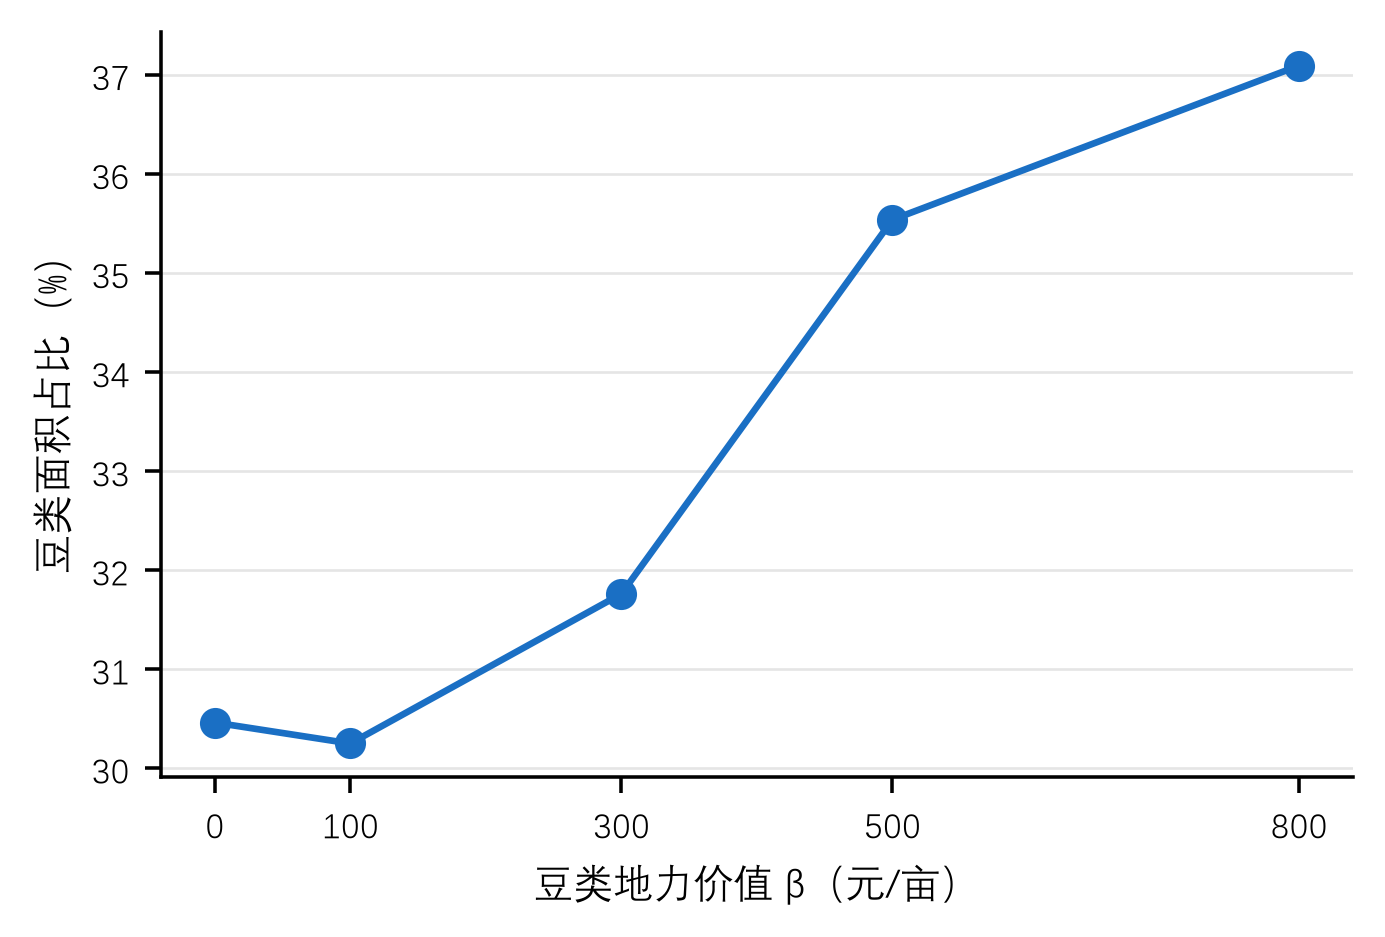
\includegraphics[width=0.70\textwidth]{figures/q1_bean_land_area_share.png}
  \caption{豆类面积占比随地力价值系数 $\beta$ 的变化}
  \label{fig:q1_bean_area}
\end{figure}

\begin{figure}[H]
  \centering
  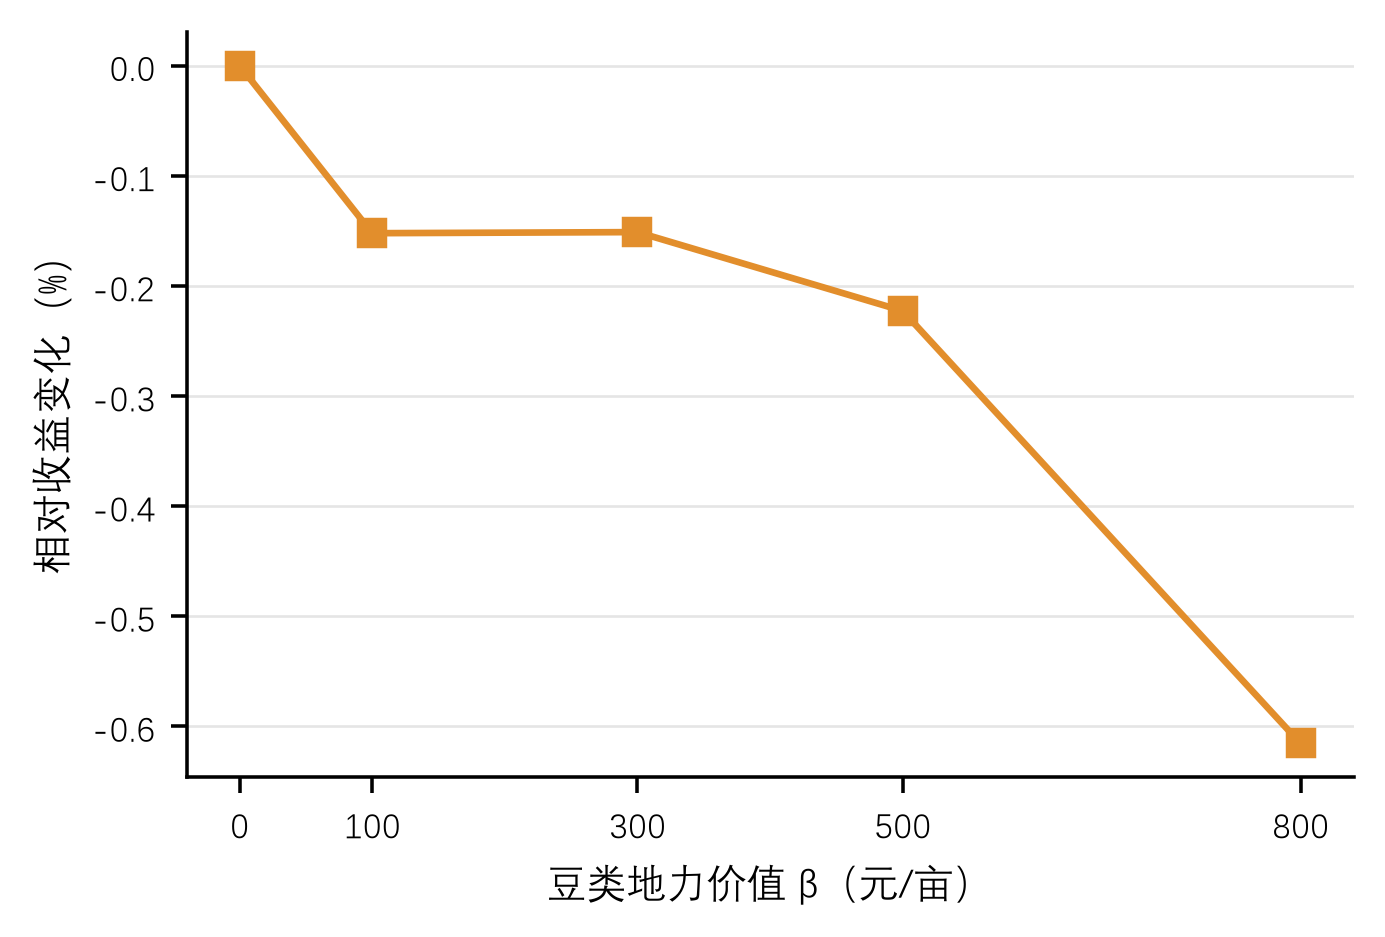
\includegraphics[width=0.70\textwidth]{figures/q1_bean_land_profit.png}
  \caption{相对收益变化随地力价值系数 $\beta$ 的变化}
  \label{fig:q1_bean_profit}
\end{figure}
